% !TeX root = ../dokumentation.tex

\chapter{Sprints}

\section{Sprint 1}
\todo{Beschreibung des Produktincrements}

\section{Ziele Sprint 1}
\todo{Ziel Sprint 1}

\section{Ergebnisse Sprint 1}

\subsection{Produktincrement}
\subsection{Charts}

\subsection{Probleme und Verbesserungen}
\todo{Retro Ergebnisse}


\subsection{Bearbeitete User Storys}
\subsubsection{SKIOS-22 POC for keycloak}
Das Ticket \enquote{SKIOS-22 POC for keycloak} hatte folgende User Story:
\begin{quotation}
    As a developer I would like to have a POC for two services using keycloak so that I’ll know how users will be managed in the future.
    Acceptance Criteria

    A backend service has an api that can get information about the logged in user

    A frontend service can create users (in any primitive way) and log in + send a request to the aformentioned endpoint
\end{quotation}
Dies wurde folgendermaßen gelöst:
\begin{quotation}
    Für den Keycloak POC wurde ein eigenes Github Repo erstellt. Darin wurde ein NodeJs und ein Angular Projekt angelegt.
    Frontend/Backend.

    Keycloak konfigurieren.
\end{quotation}
Bearbeitet von Tim Horlacher

\subsubsection{SKIOS-29 Undesigned Angular Boilerplate}
Das Ticket \enquote{SKIOS-29 Undesigned Angular Boilerplate} hatte folgende User Story:
\begin{quotation}
    As a developer I would like a boilerplate for angular to be created so that I can start work on the project.
Acceptance Criteria

    Angular Boilderplate is created with basic pages and routing

    A central structure for requests (using services) is created

    Infrastructure for passing global data (such as a username) is implemented
\end{quotation}
Dies wurde folgendermaßen gelöst:
\begin{quotation}
    I did that
    
\end{quotation}
Bearbeitet von Tim Horlacher

\subsubsection{SKIOS-31 Evaluate Core-Service}
Das Ticket \enquote{SKIOS-31 Evaluate Core-Service} hatte folgende User Story:
\begin{quotation}
    As a developer I would like to know which ORM will be used and whether or not to base our APIs around GraphQL or to stick with REST within the Core service.
Acceptance Criteria

    It is clear, what ORM to use and is documented somewhere (ex. comments of this story)

    It is clear if GraphQL is used and findings are documented somewhere aswell
\end{quotation}
Dies wurde folgendermaßen gelöst:
\begin{quotation}
    I did that
\end{quotation}
Bearbeitet von Tim Horlacher

\subsubsection{SKIOS-34 List of Participants}
Das Ticket \enquote{SKIOS-34 List of Participants} hatte folgende User Story:
\begin{quotation}
    As a professor I would like a list of group members so that I can grade the project.
Acceptance Criteria

    List is created including all 11 names and matnr.

    Said list is given to the professor
\end{quotation}
Dies wurde folgendermaßen gelöst:
\begin{quotation}
    I did that
\end{quotation}
Bearbeitet von Tim Horlacher

\subsubsection{SKIOS-52 Devcontainer Guide}
Das Ticket \enquote{SKIOS-52 Devcontainer Guide} hatte folgende User Story:
\begin{quotation}
    As a developer I guide on the usage of devcontainers for development.
Acceptance Criteria

    Create a guide in confluence

    Implement a sample devcontainer
\end{quotation}
Dies wurde folgendermaßen gelöst:
\begin{quotation}
    I did that
\end{quotation}
Bearbeitet von Tim Horlacher

\subsubsection{Ticket 1}

\subsubsection{Ticket 2}

\section{Sprint 2}
\subsection{Produktincrement}
\subsection{Charts}
\subsection{Probleme und Verbesserungen}


\subsection{Bearbeitete User Storys}

\subsubsection{SKIOS-69 Preliminary ORM}
Das Ticket \enquote{SKIOS-69 Preliminary ORM} hatte folgende User Story:
\begin{quotation}
    Als Programmierer will ich eine Datendefinition in einer Datenbank
    haben, und diese als Packet einbinden können.
\end{quotation}
Diese wurde folgendermaßen gelöst:
\begin{quotation}
Die Datendefinition wurde durch TypeORM~\parencite{web/TypeORM} dargestellt.
Diese wurde in dem Repository skiosa/orm~\parencite{git/skiosa/orm} als NPM-Package~\parencite{web/npm} abgebildet.
Es wurden die Article von RSS-Feeds in dem Schema aus Abbildung~\ref{fig:databaseORM} abgebildet.
\begin{figure}
    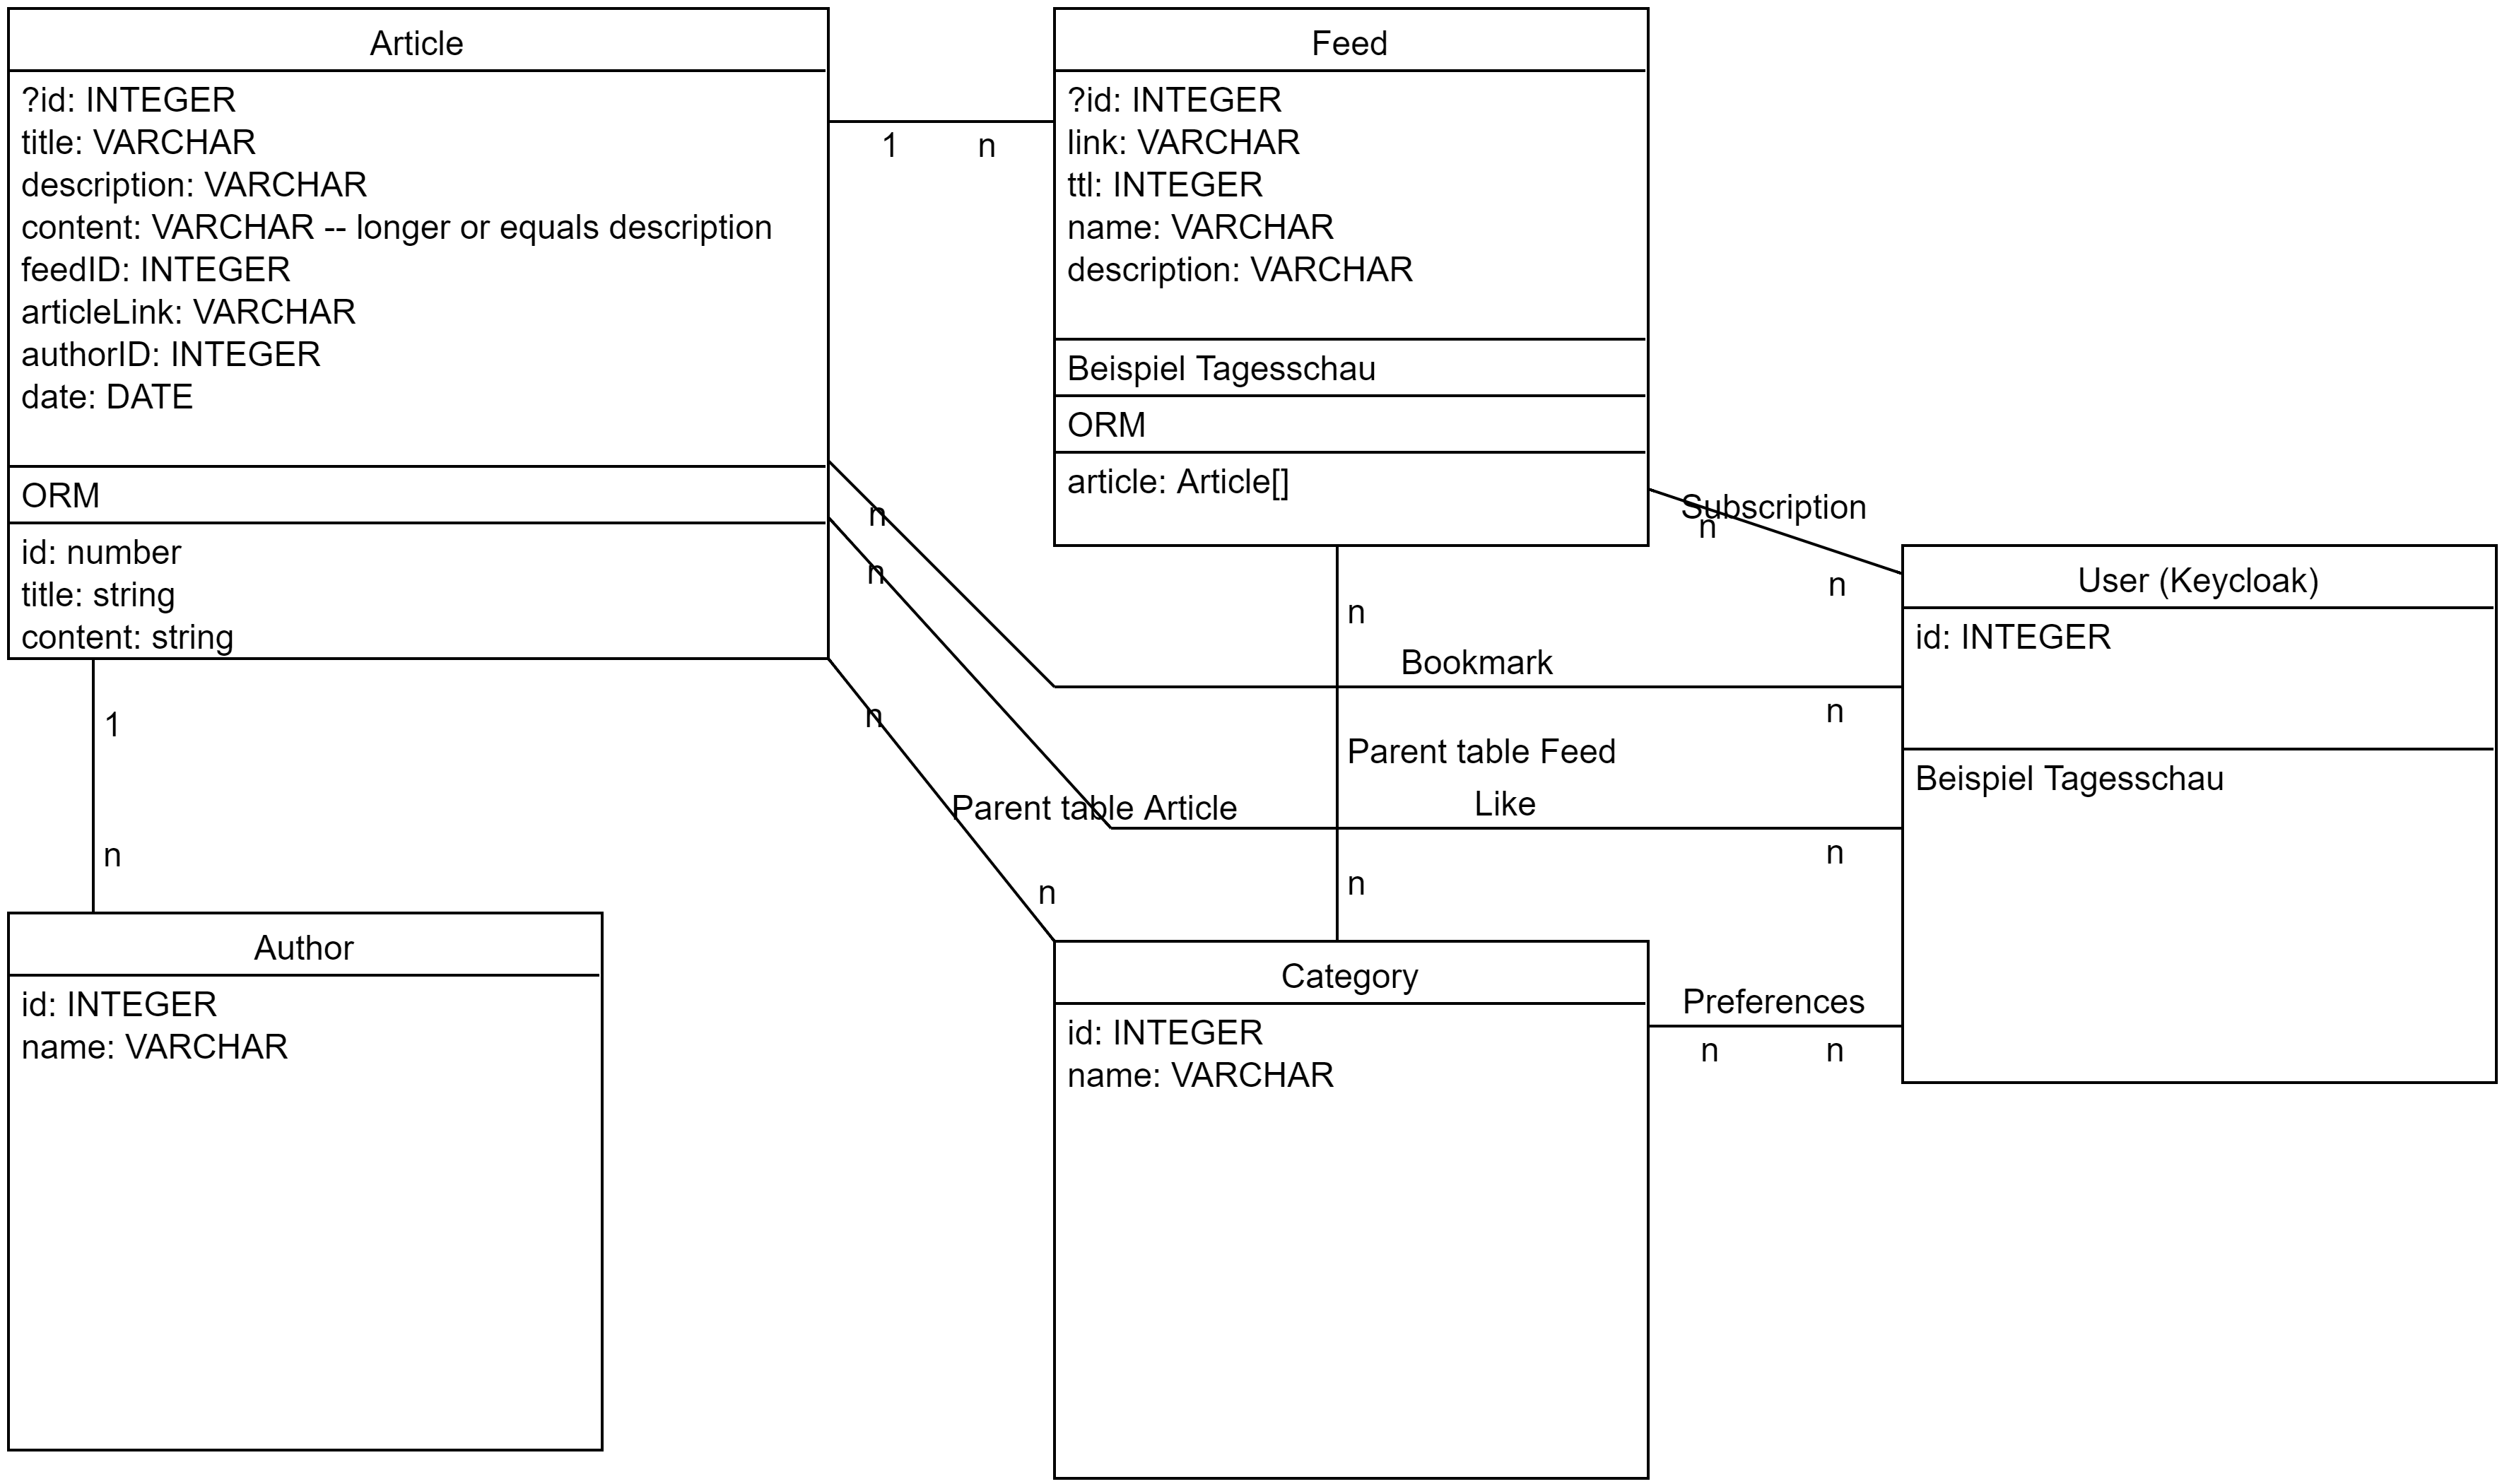
\includegraphics[width=\linewidth]{Database_Model.png}
    \caption{Datendefinition innerhalb der Datenbank}
    \label{fig:databaseORM}
\end{figure}
\end{quotation}
Bearbeitet von Jonas Eppard und Tim Horlacher.

\subsubsection{SKIOS-92 Initialize Keycloak}
Das Ticket \enquote{SKIOS-92 Initialize Keycloak} hatte folgende User Story:
\begin{quotation}
    create realm (test, prod)

    client frontend

    client backend

    create roles

    creat user properties
\end{quotation}
Dies wurde folgendermaßen gelöst:
\begin{quotation}
    I did that.
\end{quotation}
Bearbeitet von Tim Horlacher

\subsubsection{SKIOS-93 Document Submission Guideline}
Das Ticket \enquote{SKIOS-93 Document Submission Guideline} hatte folgende User Story:
\begin{quotation}
    As a team member i would like to know what should be documented.
Acceptance Criteria

    A confluence page documents what should be documented
\end{quotation}
Dies wurde folgendermaßen gelöst:
\begin{quotation}
    I did that
\end{quotation}
Bearbeitet von Tim Horlacher

\section{Sprint 3}

\subsection{Produktincrement}
\subsection{Charts}
\subsection{Probleme und Verbesserungen}


\subsection{Bearbeitete User Storys}
\subsubsection{SKIOS-116 Structure and table of contents for submission (\LaTeX)}
Das Ticket \enquote{SKIOS-116 Structure and table of contents for submission (\LaTeX)}
hatte folgende User Story:
\begin{quotation}
    As a team member, I would like to have a rough structure to orient myself while writing our submission documentation.\\
    For this story, please read the requirements and guidelines set out by Garidis and develop a rough idea on how to structure our \LaTeX project.\\
    \textbf{Acceptance Criteria}
    \begin{itemize}
        \item Table of contents is created (with \textbackslash{}section, \textbackslash{}subsection, etc.) in \LaTeX
        \item Structure reflects guidelines of Garidis
        \item Structure is explained in confluence page
        \item Existing \LaTeX~stories have a defined place where their pages will go
    \end{itemize}
\end{quotation}
Dies wurde folgendermaßen gelöst:
\begin{quotation}
    Es wurde die Struktur dieses \LaTeX-Dokuments angelegt. Hierbei musste nur das Inhaltsverzeichnis
    angelegt werden, da das \LaTeX-Template schon vorhanden war.
    Die Verwendung wurde in Confluence dokumentiert.
\end{quotation}
Bearbeitet von Jonas Eppard.
